\begin{figure}[!t]
    \centering
    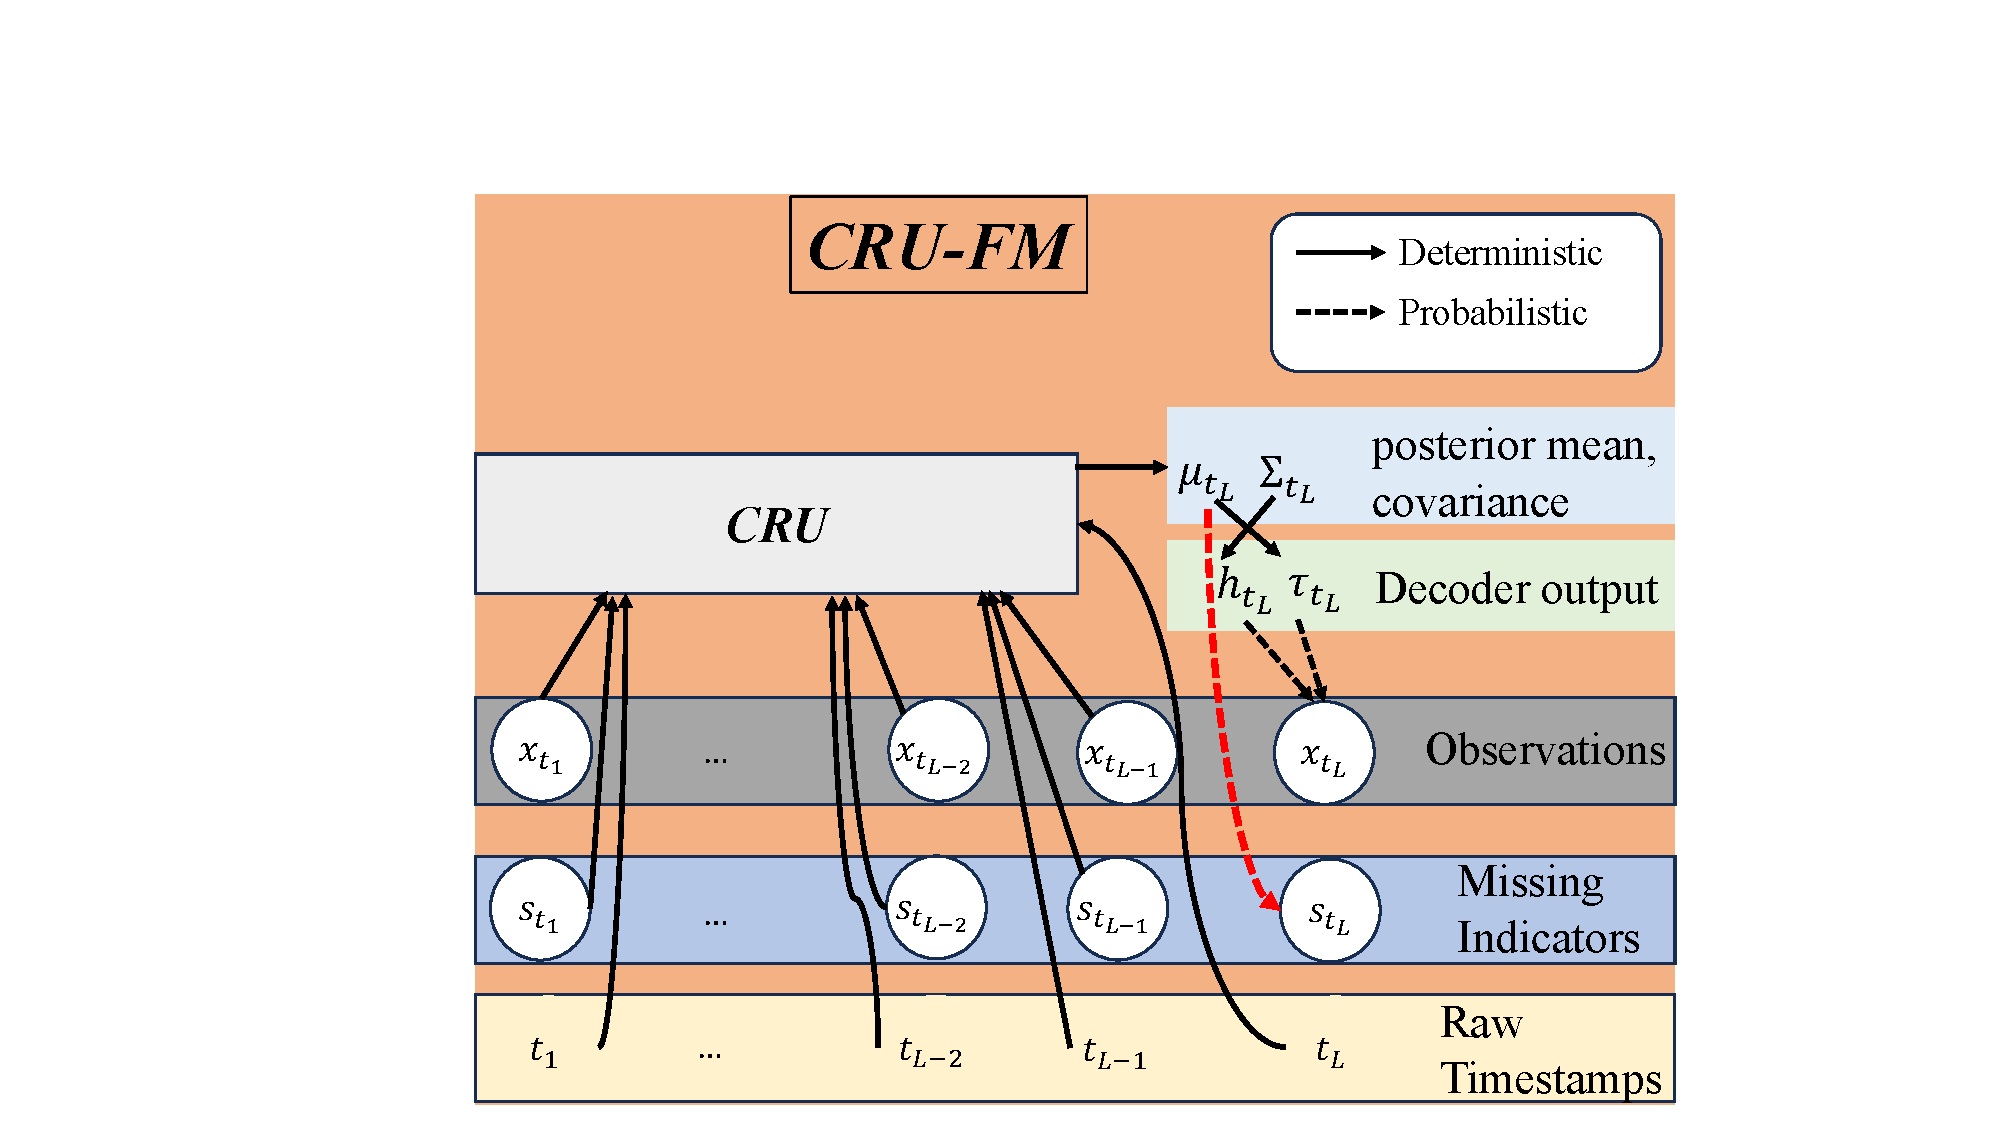
\includegraphics[width=0.9\textwidth]{content/chapters/irregular_time_series_data_driven_missingness/figures/cru_fm_diagram.pdf}
    \caption[Diagram of our proposed CRU-FM model]{Diagram of our CRU-FM model (Sec.~\ref{sec:CRU_gen_model}). We show the extrapolation generative process for data vector $x_{t_L}$ and binary seen/missing indicator $s_{t_L}$ at time $t_L$, conditioning on previous $x_{t_1:t_{L-1}}, s_{t_1:t_{L-1}}$.
    The red line highlights our contribution: a distribution on $s_{t_L}$ that is data-dependent and thus suitable for MAR settings. Dashed lines point to values that are sampled from a distribution, not deterministically computed from predecessors. 
    }%endcaption
    \label{fig:generative_model}
    % \vspace{-.7cm} %% HACK
\end{figure}
